\section{Discussion} 



\begin{itemize}

    \item

        Discuss that we would have liked to train an RNN on the character limit
        but that we did not have the computation power.

    \item

        Discuss how comparable our results will be with data in the real world.
        We had no texts written by actual ghost writers so we have no idea how
        our networks would perform on such texts.

\end{itemize}

\label{sec:discussion} Looking at the results presented in \ref{sec:results},
is apparent that we've hit at several points of the spectrum. While none of our
methods did achieve the sub 10\% accusation error on the test set, that MaCom
required, we believe that some of the methods does in fact show promise within
the NLP field. The best performing method that we've tested, is without a doubt
the \ref{conv-char-NN} neural network. 

\subsection{Teacher Feedback}

In our introduction we reported that we wanted to look at what kind of feedback
we could give to teachers in conjunction with the bare predictions. As explained
earlier the system is not meant to be the final judge of which students are
cheating but are rather meant as a support system for teachers that are
already suspicious. We have looked at what kind of feedback we could give to
teachers. We have focused on the \gls{conv-char-NN} network since it performed
best on the test dataset. We have previously looked at the output of the
feature extraction layer to obtain information on what a specific network
were looking at. We wanted to do something similar for teacher feedback.
Recall that \gls{conv-char-NN} started with a convolutional layer followed
by a max pool layer. We therefore know that the larger the output of the
convolutional layer the more important that particular character sequence
is. The output of the feature extraction can be thought of as in Figure
\ref{fig:feature_extraction_output_example}. Each filter gives a single
output that is the maximum output in any filter position. The combining function
for the third network was the absolute difference. That means that when we
are comparing $t$ and $t'$. That means that the output of the combination
will be high for a particular filter iff the maximum output of that filter is
significantly different for $t$ and $t'$.

\begin{figure}
    \centering
    \textbf{Teacher Feedback Script Example}\par\medskip
    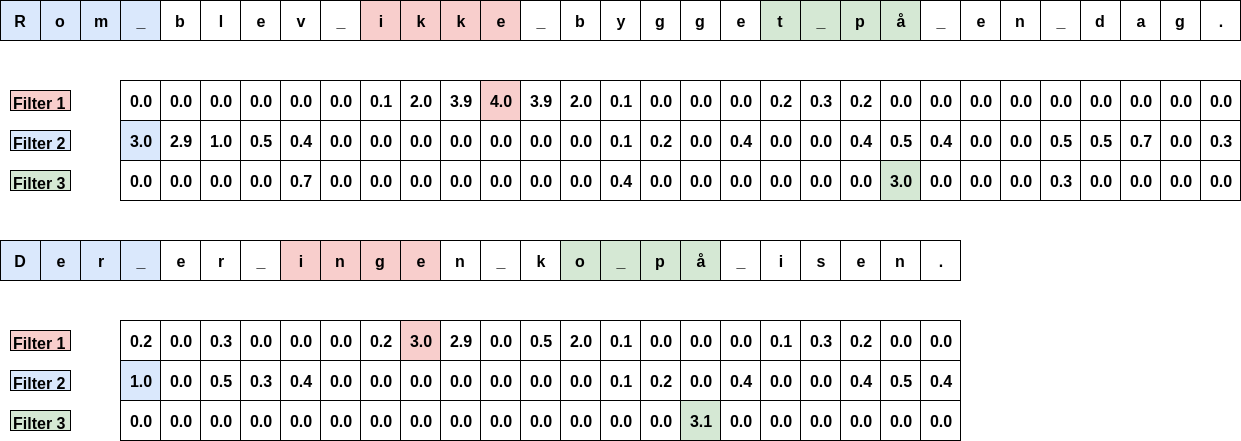
\includegraphics[width=\textwidth]{./pictures/discussion/teacher_feedback_example.png}
    \caption{Illustrates our script that gives feedback to teachers. The
        particular network used in this example only has three filters. The
        three filters maximum activations are shown in three different colors
        for the two texts they are comparing. The first filter looks for
        negative qualifiers. Therefore it reacts strongly to both the Danish
        word "ikke" (not) and the Danish word "ngen" (noone). The second filter
        looks for city names so it reacts strongly to the string "Rom " (Rome)
        but less strongly to "Der " (not a city name) even though it looks like
        a city name. The third filter reacts to phrases that contains the word
        "p\aa " (on) and therefore reacts about the same to both texts.}
    \label{fig:feature_extraction_output_example}
\end{figure}

% TODO: Maybe the figure here (fig:feature_extraction_output_example)?

It is hard to know exactly what the following layers does with the absolute
difference but we feel that it is a fair assumption that the largest filter
differences translates to the most important differences. The feedback system
we implemented for teachers takes an author $\alpha$, text $t$ and $n \in
\mathbb{N}^+$ and outputs the $n$ largest differences between each $t' \in
T_\alpha$ and $t$. The idea is that the when our system reports a negative the
teacher can ask for feedback from the system. The teacher will then get a list
of the $n$ greatest differences between each of the texts and can use that
information to argue against the student.

As an example we ran our system on a random author and a text that that author
did not write. The whole output of three different texts can be seen in Appendix
\ref{subsec:teacher_feedback_text_comparisons} through \ref{TODO}. We have shown
a truncated output in Table \ref{tab:teacher_feedback_output}.

\begin{table}
    \begin{tabular}{llll}
        \textbf{Filter} & \textbf{Activation Text 1} &
        \textbf{Activation Text 2} & \textbf{Difference} \\
        \hline
        426 & \verb'"; ”Hvis "'  & \verb'". Et kla"' & $|2.82 - 4.57| = 1.75$ \\
        71  & \verb'"dem; Nia"'  & \verb'"der skri"' & $|4.64 - 3.16| = 1.45$ \\
        549 & \verb'". Jeg vi"'  & \verb'". Her is"' & $|2.61 - 4.02| = 1.41$ \\
        288 & \verb'" 2 af 2\n"' & \verb'"og refle"' & $|4.90 - 3.53| = 1.37$ \\
        496 & \verb'" udseend"'  & \verb'"vad litt"' & $|2.78 - 4.12| = 1.34$ \\
        33  & \verb'"et sind."'  & \verb'"risning,"' & $|3.05 - 4.36| = 1.31$ \\
        460 & \verb'" 2 af 2\n"' & \verb'" krig og"' & $|3.69 - 2.43| = 1.26$ \\
        514 & \verb'", derfor"'  & \verb'", i forb"' & $|3.82 - 5.06| = 1.24$ \\
        531 & \verb'" om, for"'  & \verb'" om, hva"' & $|4.64 - 5.84| = 1.20$ \\
        458 & \verb'"Derudove"'  & \verb'"derfor b"' & $|4.31 - 3.13| = 1.18$ \\
        \\
        261 & \verb'".\n\n\n"'   & \verb'"– de"'     & $|1.72 - 2.70| = 0.98$ \\
        484 & \verb'"lv; "'      & \verb'" dét"'     & $|2.02 - 2.96| = 0.94$ \\
        17  & \verb'"st ”"'      & \verb'"gt; "'     & $|2.57 - 3.45| = 0.88$ \\
        145 & \verb'"ndet"'      & \verb'" Det"'     & $|2.37 - 3.25| = 0.88$ \\
        299 & \verb'"osse"'      & \verb'"– de"'     & $|3.12 - 3.98| = 0.86$ \\
        477 & \verb'"f 2\n"'     & \verb'"v og"'     & $|3.05 - 2.20| = 0.85$ \\
        421 & \verb'" 13."'      & \verb'" vel"'     & $|3.03 - 2.19| = 0.84$ \\
        434 & \verb'"am; "'      & \verb'" dét"'     & $|1.18 - 2.00| = 0.82$ \\
        27  & \verb'"n to"'      & \verb'"Dett"'     & $|2.20 - 2.99| = 0.79$ \\
        445 & \verb'" om,"'      & \verb'" – S"'     & $|2.51 - 3.27| = 0.76$ \\
    \end{tabular}
    \caption{Shows the 10 most different activations of convolutional filters on
        two different texts. Both the 10 most different activations for the
        filter of size 8 and size 4 is shown. The strings that produced the
        activation are shown and the actual activations are shown to the right.}
    \label{tab:teacher_feedback_output}
\end{table}



